% !TeX program = pdflatex
\documentclass[10pt,aspectratio=169]{beamer}
\usepackage{iftex}
\ifPDFTeX
  \usepackage[T5]{fontenc}
  \usepackage[utf8]{inputenc}
  \usepackage{lmodern}
\else
  \usepackage{fontspec}
  \setsansfont{texgyreheros}[Extension=.otf,UprightFont=*-regular,
    BoldFont=*-bold,ItalicFont=*-italic,BoldItalicFont=*-bolditalic]
\fi

% ===== PRESENTATION METADATA =====
\newcommand{\CourseName}{AIT3012 Neuroscience - Course Mini Project}
\newcommand{\ProjectTitle}{Single-trial P300 classification}
\newcommand{\ProjectSubtitle}{Feature-based machine learning and EEGNet in a visual oddball task}
\newcommand{\Instructor}{Prof. Guy Nagels, VUB}
\newcommand{\TeachingAssistants}{Trần Quốc Sáng, Nguyễn Tiến Dũng}
\newcommand{\TeamMembers}{Nguyễn Văn Vũ, Thái Nguyễn Hoàng Bách, Trương Huy Hoàng,\\Nguyễn Công Kiên, Nguyễn Việt Đức, Đồng Minh Đức}
\newcommand{\PresentationDate}{November 2026}
\newcommand{\InstituteName}{VNU University of Engineering and Technology - Institute of Artificial Intelligence}

% ===== BEAMER THEME & STYLING =====
\usepackage{tikz}
\usetikzlibrary{arrows.meta,positioning,calc}
\usepackage{graphicx,booktabs,tabularx,array,amsmath,amssymb}
\graphicspath{{images/}{figures/}}

\definecolor{Navy}{HTML}{00346F}
\definecolor{DeepNavy}{HTML}{002C6B}
\definecolor{TitleNavy}{HTML}{253E6C}
\definecolor{AccentRed}{HTML}{FF544F}
\definecolor{AccentBlue}{HTML}{538CD5}
\definecolor{PaleBlue}{HTML}{EEF4FA}
\definecolor{Muted}{HTML}{586879}
\definecolor{Teal}{HTML}{0097A7}

\setbeamercolor{normal text}{fg=black,bg=white}
\setbeamercolor{structure}{fg=Navy}
\setbeamercolor{frametitle}{fg=black,bg=white}
\setbeamercolor{footline}{fg=white,bg=Navy}
\setbeamercolor{block title}{fg=Navy,bg=PaleBlue}
\setbeamercolor{block body}{fg=black,bg=PaleBlue}
\setbeamerfont{normal text}{size=\fontsize{9.2}{11.5}\selectfont}
\setbeamerfont{block title}{size=\small,series=\bfseries}
\setbeamerfont{block body}{size=\scriptsize}
\setbeamerfont{footline}{size=\fontsize{6.3}{7}\selectfont,series=\bfseries}
\setbeamersize{text margin left=7mm,text margin right=7mm}
\setbeamertemplate{navigation symbols}{}
\setbeamertemplate{itemize item}{\raisebox{0.15ex}{\scriptsize\textbullet}}
\setbeamertemplate{itemize subitem}{\scriptsize$\circ$}
\setbeamercolor{itemize item}{fg=Navy}
\setbeamercolor{itemize subitem}{fg=Navy}
\setbeamertemplate{enumerate items}[default]
\setbeamertemplate{blocks}[rounded][shadow=false]

\newcommand{\sectionindex}{01}
\newif\ifcoverpage
\coverpagefalse

\newcommand{\headerlogos}{%
  
\includegraphics[height=7.2mm]{logo_uet.png}\hspace{1.5mm}%
  
\includegraphics[height=7.2mm]{logo_ai.png}}

\setbeamertemplate{background}{%
  \begin{tikzpicture}[remember picture,overlay]
    \ifcoverpage
      \node[anchor=north west,inner sep=0pt] at ([xshift=6mm,yshift=-4mm]current page.north west)
        {\headerlogos\hspace{3mm}\textcolor{DeepNavy}{\bfseries\fontsize{8.5}{10}\selectfont VNU-UET \textbar\ Institute of Artificial Intelligence}};
    \else
      \node[anchor=north east,inner sep=0pt] at ([xshift=-5mm,yshift=-3mm]current page.north east) {\headerlogos};
    \fi
  \end{tikzpicture}}

\setbeamertemplate{frametitle}{%
  \vskip1mm
  \begin{tikzpicture}
    \path[use as bounding box] (0,0) rectangle (\textwidth,11.5mm);
    \node[anchor=west,inner sep=0pt,font=\bfseries\fontsize{10.5}{12.5}\selectfont,text=Navy] at (0,7mm) {\sectionindex};
    \draw[AccentRed,line width=1.1pt] (7.5mm,6mm)--(7.5mm,10.5mm);
    \draw[AccentBlue,line width=1.1pt] (7.5mm,0.8mm)--(7.5mm,6mm);
    \node[anchor=west,inner sep=0pt,font=\bfseries\fontsize{11.5}{13.5}\selectfont,text=DeepNavy] at (9.5mm,7.5mm) {\insertframetitle};
    \node[anchor=west,inner sep=0pt,text=Muted,font=\itshape\fontsize{8}{10}\selectfont] at (9.5mm,2.4mm) {\insertframesubtitle};
  \end{tikzpicture}}

\setbeamertemplate{footline}{%
  \begin{beamercolorbox}[wd=\paperwidth,ht=2.8mm,dp=1mm,leftskip=4mm,rightskip=4mm]{footline}
    \usebeamerfont{footline}\InstituteName\hfill\insertframenumber\,/\,\inserttotalframenumber
  \end{beamercolorbox}}

\newcommand{\source}[1]{\par\vspace{0.6mm}{\fontsize{6.2}{7.5}\selectfont\color{Muted}Source: #1.\par}}
\newcommand{\takeaway}[1]{\par\vspace{0.8mm}%
  \begingroup\setlength{\fboxsep}{1.2mm}\colorbox{PaleBlue}{%
    \parbox{\dimexpr\linewidth-2.4mm\relax}{\fontsize{8}{9.6}\selectfont\color{Navy}#1}}\endgroup\par}

\newcommand{\notebook}{%
  
\begin{tikzpicture}[x=1mm,y=1mm]
    \fill[AccentBlue!20,rounded corners=2mm] (1,-1) rectangle (31,34);
    \fill[Navy,rounded corners=2mm] (0,0) rectangle (30,35);
    \fill[white] (4,3) rectangle (27,32);
    \fill[Teal] (1,0) rectangle (5,35);
    \foreach \y in {10,15,20,25}{\draw[AccentBlue!45,line width=0.5pt] (9,\y)--(23,\y);}
    \fill[AccentRed] (20,0)--(20,-6)--(22,-4)--(24,-6)--(24,0)--cycle;
    \begin{scope}[shift={(5,42)},rotate=-8]
      \fill[orange!85!yellow,rounded corners=0.5mm] (0,0) rectangle (29,2.5);
      \fill[AccentRed] (-3,0) rectangle (0,2.5);
      \fill[Muted] (29,0)--(32,1.25)--(29,2.5)--cycle;
    \end{scope}
  \end{tikzpicture}}

\hypersetup{colorlinks=true,urlcolor=Navy,linkcolor=Navy}

\title[Single-trial P300 classification]{\ProjectTitle}
\subtitle{\ProjectSubtitle}
\author{\TeamMembers}
\institute{\InstituteName}
\date{\PresentationDate}

\begin{document}

% ==============================================================================
% SLIDE 1: TITLE SLIDE (ACADEMIC COURSE PROJECT DEFENSE)
% ==============================================================================
\coverpagetrue
\begin{frame}
  \vspace{7mm}
  {\color{AccentRed}\fontsize{9}{11}\selectfont\bfseries\CourseName}\par
  \vspace{2.5mm}
  {\raggedright\color{TitleNavy}\bfseries\fontsize{18}{22}\selectfont
    Single-trial P300 classification\par}
  \vspace{1.5mm}
  {\color{Muted}\fontsize{9.5}{12}\selectfont
    Feature-based machine learning and EEGNet in a visual oddball task\par}
  \vspace{2mm}
  {\color{AccentRed}\rule{0.95\linewidth}{0.8pt}}\par
  \vspace{3.5mm}
  \begin{columns}[T,onlytextwidth]
    \begin{column}{0.48\textwidth}
      {\scriptsize\color{Muted}Academic course:}\hspace{1mm}{\scriptsize\color{Navy}AIT3012 Neuroscience}\par
      \vspace{1mm}
      {\scriptsize\color{Muted}Instructor:}\hspace{1mm}{\scriptsize\color{Navy}\Instructor}\par
      \vspace{1mm}
      {\scriptsize\color{Muted}Teaching assistants:}\hspace{1mm}{\scriptsize\color{Navy}\TeachingAssistants}\par
      \vspace{1mm}
      {\scriptsize\color{Muted}Institution:}\hspace{1mm}{\scriptsize\color{Navy}\InstituteName}
    \end{column}
    \begin{column}{0.48\textwidth}
      {\scriptsize\color{Muted}Student team:}\par
      \vspace{1mm}
      {\scriptsize\color{DeepNavy}
      \begin{tabular}{ll}
      Nguyễn Văn Vũ & Thái Nguyễn Hoàng Bách \\
      Trương Huy Hoàng & Nguyễn Công Kiên \\
      Nguyễn Việt Đức & Đồng Minh Đức
      \end{tabular}}
    \end{column}
  \end{columns}
\end{frame}
\coverpagefalse

% ==============================================================================
% SLIDE 2: RESEARCH CONTEXT & THE THREE QUESTIONS
% ==============================================================================
\renewcommand{\sectionindex}{01}
\begin{frame}{Research context and the three core questions}
  \framesubtitle{Evaluating single-trial brain response classification in visual oddball EEG}
  \begin{columns}[T,onlytextwidth]
    \begin{column}{0.43\textwidth}
      \textbf{Project overview}
      \begin{itemize}
        \setlength{\itemsep}{2mm}
        \scriptsize
        \item Dataset: Nencki-Symfonia visual oddball task with 42 healthy participants and 128 channels.
        \item Task: classify target versus frequent standard stimuli from individual single trials.
        \item Challenge: target response (${\approx}7\,\mu\text{V}$) is buried in ongoing EEG noise (${\pm}50\,\mu\text{V}$).
        \item Analysis cohort: 39 task-compliant participants and 21,878 correct trials.
      \end{itemize}
    \end{column}
    \begin{column}{0.54\textwidth}
      \textbf{Three research questions set by Prof. Guy Nagels}
      \begin{enumerate}
        \setlength{\itemsep}{2mm}
        \scriptsize
        \item \textbf{Research question 1}: What is the best single-trial classification result for frequent versus target stimuli?
        \item \textbf{Research question 2}: Is deep learning better for single-trial classification compared to standard machine learning techniques?
        \item \textbf{Research question 3}: Are the features that the deep learning model discovers explainable? If deep learning is not better, what is the reason?
      \end{enumerate}
    \end{column}
  \end{columns}
  \vspace{1mm}
  \takeaway{Our 10-minute presentation directly answers these three questions using rigorous cross-subject benchmarks and interpretability analysis.}
  \source{Lecture slide 142; Dzianok et al., GigaScience (2022)}
\end{frame}

% ==============================================================================
% SLIDE 3: NEUROPHYSIOLOGICAL BASIS (POLICH MODEL)
% ==============================================================================
\renewcommand{\sectionindex}{02}
\begin{frame}{P300 framework (Polich, 2007) and difference waves}
  \framesubtitle{Target and distractor contrasts in an easy visual oddball task}
  \begin{columns}[c,onlytextwidth]
    \begin{column}{0.38\textwidth}
      \textbf{Integrative theory (Polich, 2007)}
      \begin{itemize}
        \setlength{\itemsep}{1.5mm}
        \scriptsize
        \item P3b: task-relevant context updating to targets with a parietal maximum ($Pz > Fz$).
        \item Fronto-central P3a appears mainly when target--standard discrimination is difficult; easy tasks elicit a parietal distractor P3.
      \end{itemize}
      \vspace{1.8mm}
      \textbf{Observed difference waves (300--500~ms)}
      \begin{itemize}
        \setlength{\itemsep}{1.3mm}
        \scriptsize
        \item Target $-$ standard: strong parietal P3b ($+5.05\,\mu\text{V}$ at Pz).
        \item Distractor $-$ standard: also predominantly parietal ($+3.54\,\mu\text{V}$ at Pz; $-1.06\,\mu\text{V}$ at Fz) --- not a canonical frontal P3a.
        \item Relative anterior shift vs.\ targets in 26/39 participants ($+1.43 \pm 2.46\,\mu\text{V}$).
      \end{itemize}
    \end{column}
    \begin{column}{0.60\textwidth}
      \begin{center}
        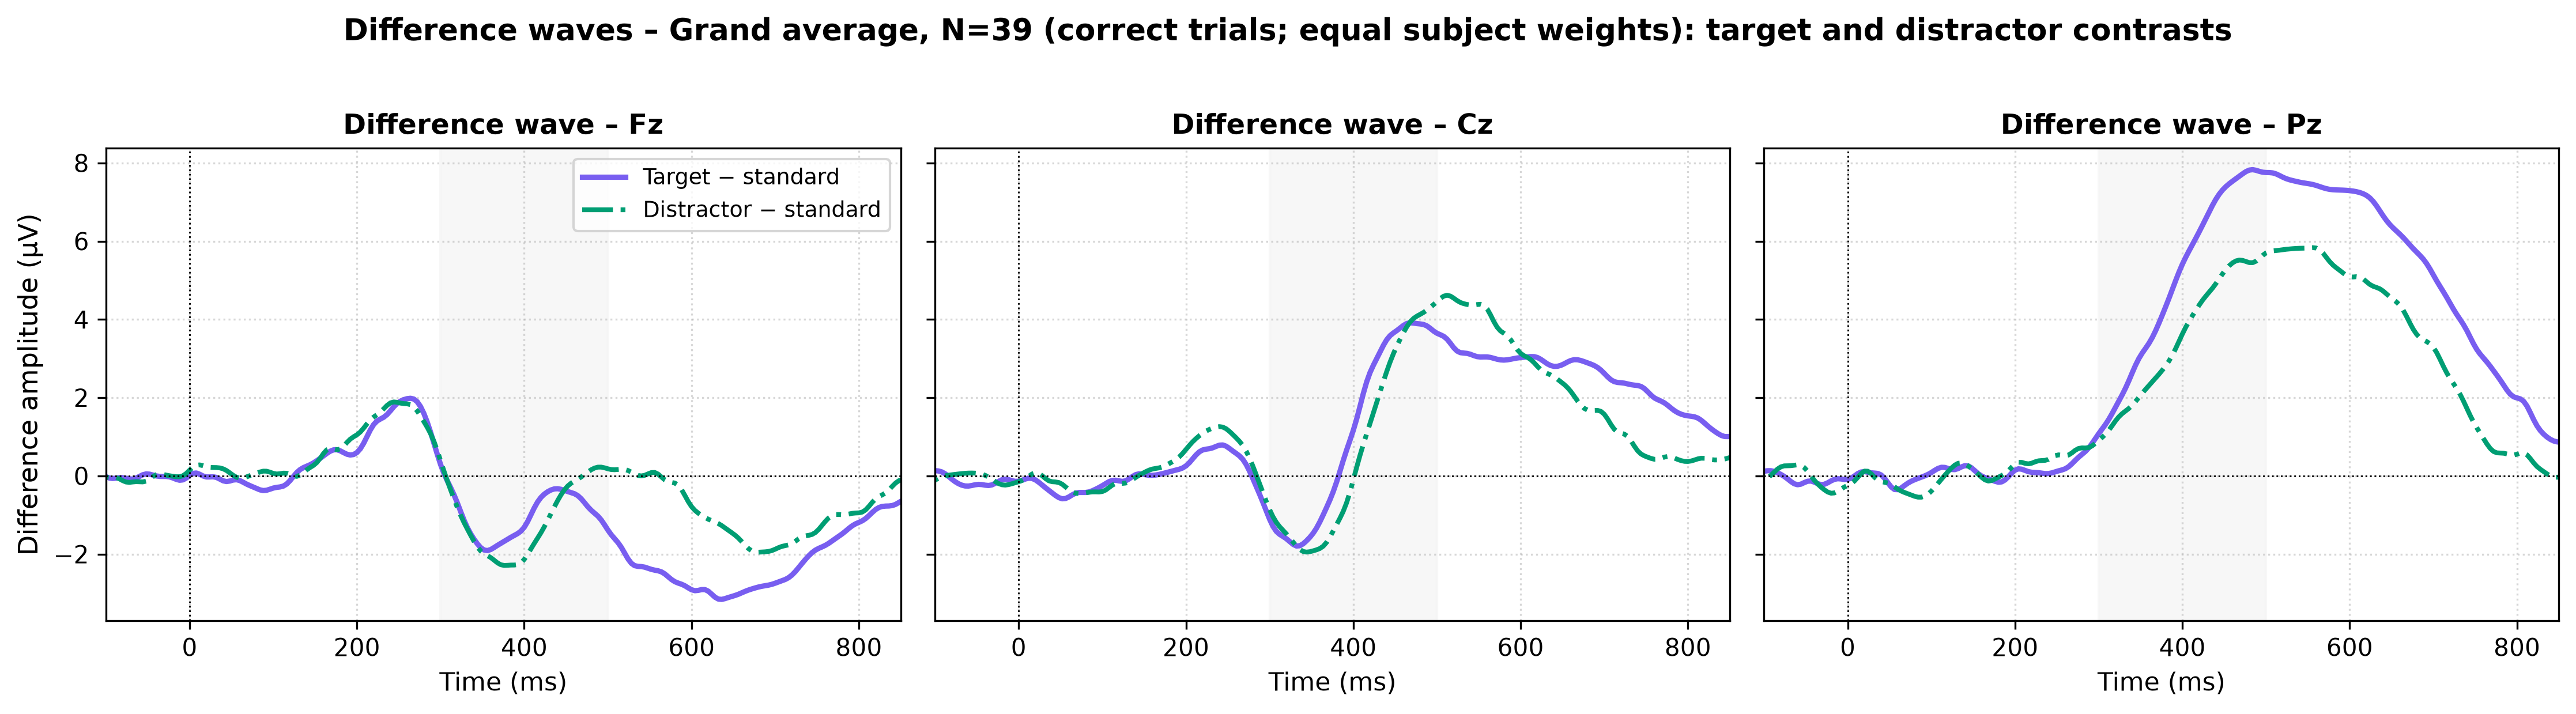
\includegraphics[width=0.98\linewidth,height=52mm,keepaspectratio]{grand_average_difference_waves.png}
      \end{center}
      \source{Figure 4: Group difference waves at Fz, Cz, and Pz across 39 compliant participants}
    \end{column}
  \end{columns}
\end{frame}

% ==============================================================================
% SLIDE 4: GROUP ERP & ODDBALL EFFECT
% ==============================================================================
\begin{frame}{Group event-related potentials and parietal effect}
  \framesubtitle{Equally weighted group average confirms massive parietal oddball effect}
  \begin{columns}[c,onlytextwidth]
    \begin{column}{0.61\textwidth}
      \begin{center}
        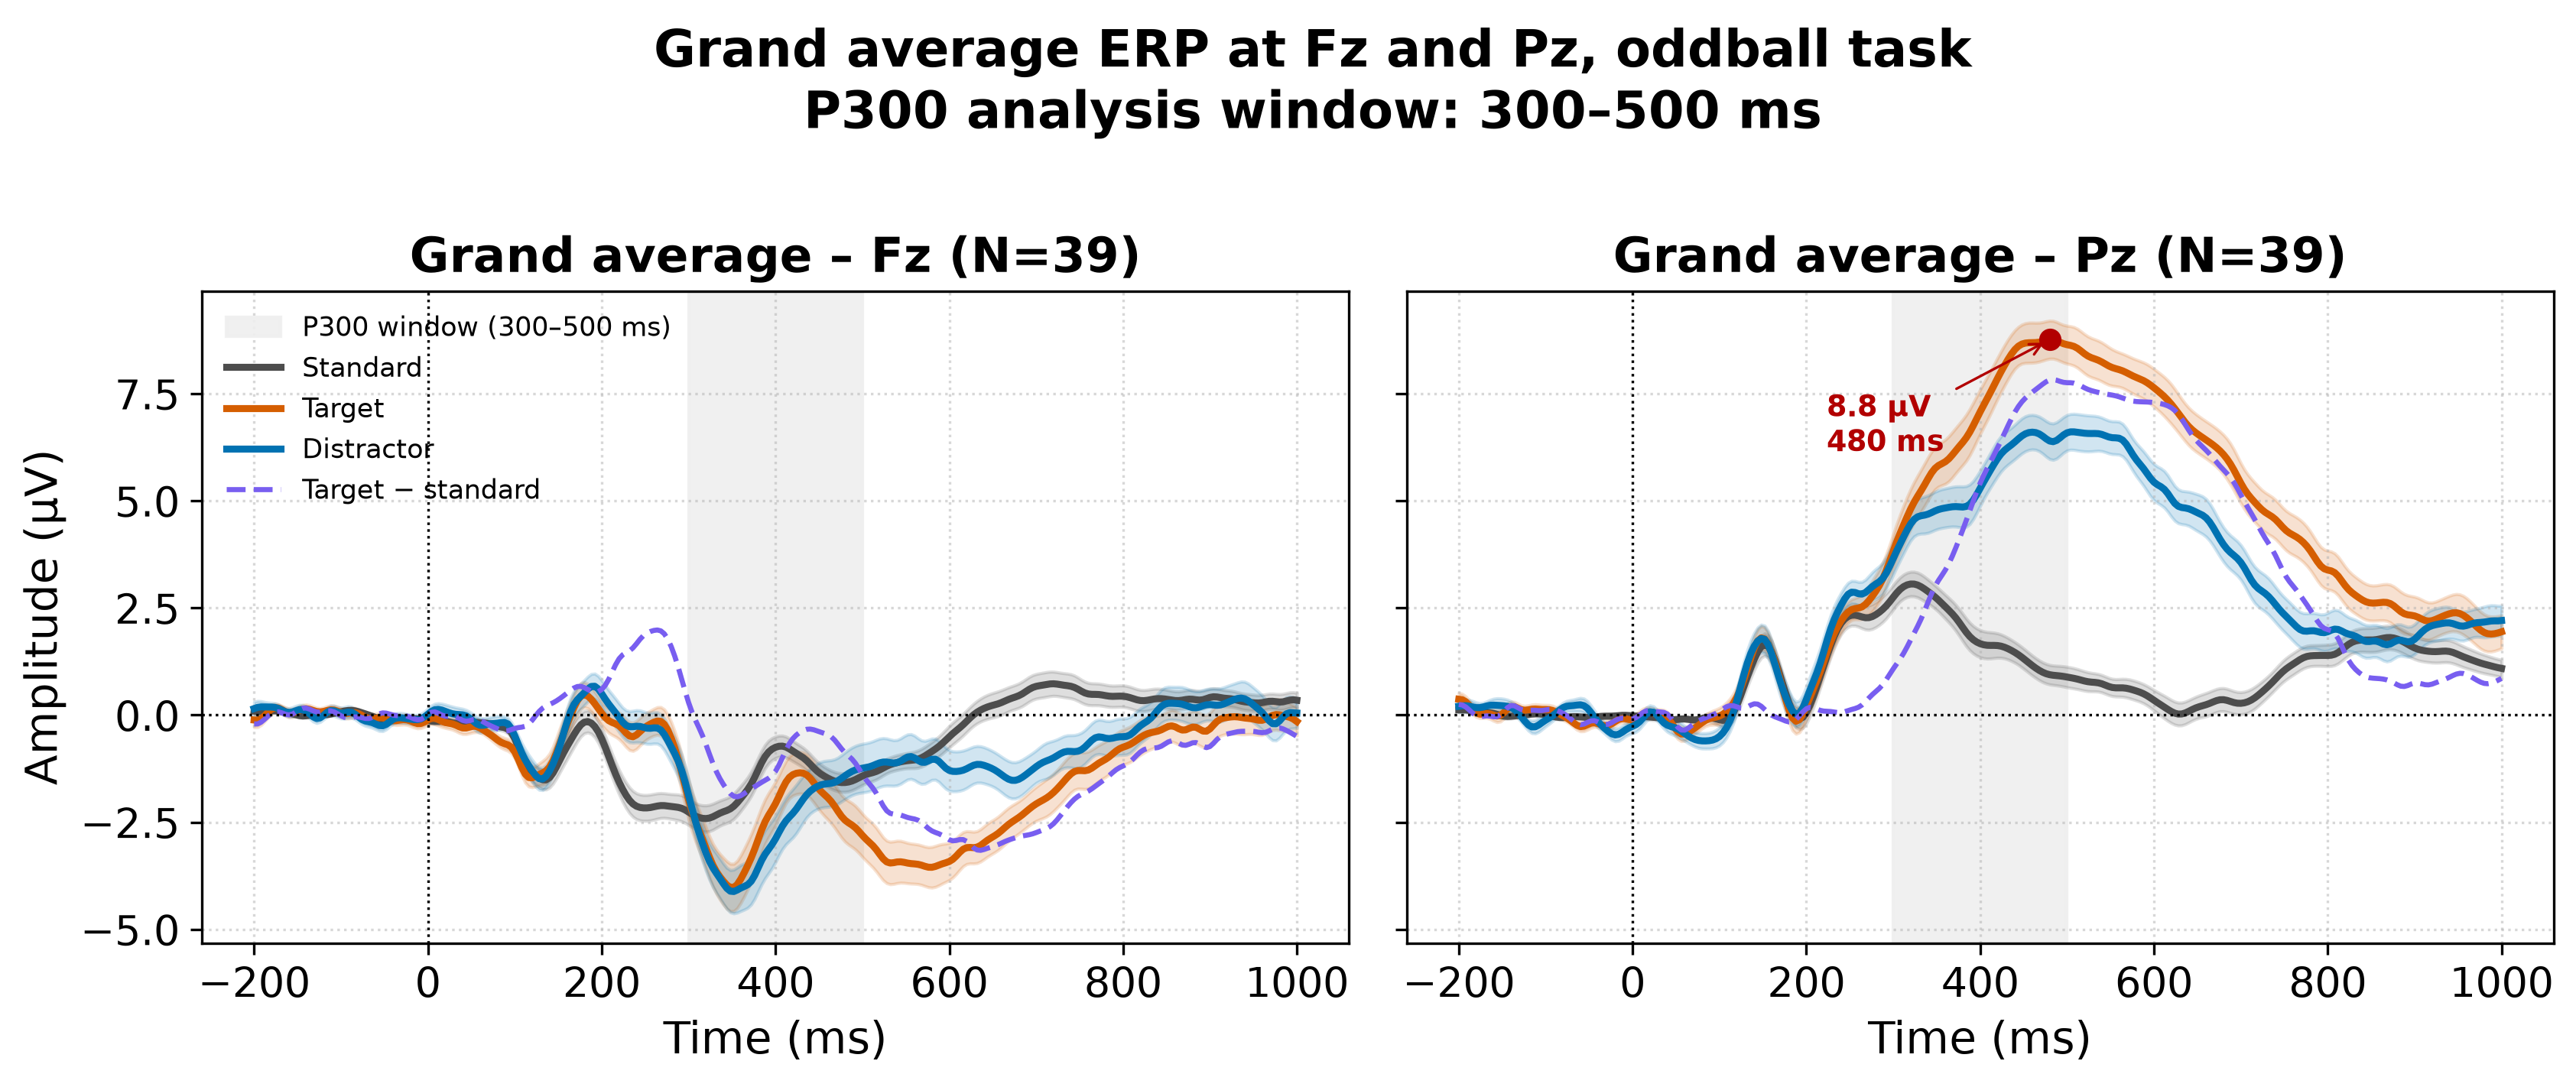
\includegraphics[width=0.98\linewidth,height=50mm,keepaspectratio]{grand_average_fz_pz.png}
      \end{center}
      \source{Figure 2: Equal-participant-weight ERPs at Fz and Pz across 39 participants}
    \end{column}
    \begin{column}{0.37\textwidth}
      \textbf{Quantitative ERP findings}
      \begin{itemize}
        \setlength{\itemsep}{2mm}
        \scriptsize
        \item Target Pz mean reaches $6.97 \pm 2.74\,\mu\text{V}$ compared to $1.92 \pm 1.49\,\mu\text{V}$ for standard (300--500 ms).
        \item Target minus standard difference is $5.05 \pm 2.28\,\mu\text{V}$ in 300--500 ms.
        \item Statistical significance: $t(38) = 13.82,\ p = 2.14 \times 10^{-16}$, Cohen's $d_z = 2.21$.
        \item Parietal gradient: 39 of 39 compliant participants satisfy target $Pz > Fz$.
        \item Reaction time ($542.1 \pm 65.5\text{ ms}$) negatively correlates with Pz amplitude ($r = -0.493,\ p = 0.00144$).
      \end{itemize}
    \end{column}
  \end{columns}
\end{frame}

% ==============================================================================
% SLIDE 5: PREPROCESSING PIPELINE & QUALITY CONTROL
% ==============================================================================
\renewcommand{\sectionindex}{03}
\begin{frame}{Standardized preprocessing pipeline and quality control}
  \framesubtitle{Automated artifact attenuation with objective participant inclusion criteria}
  \begin{center}
    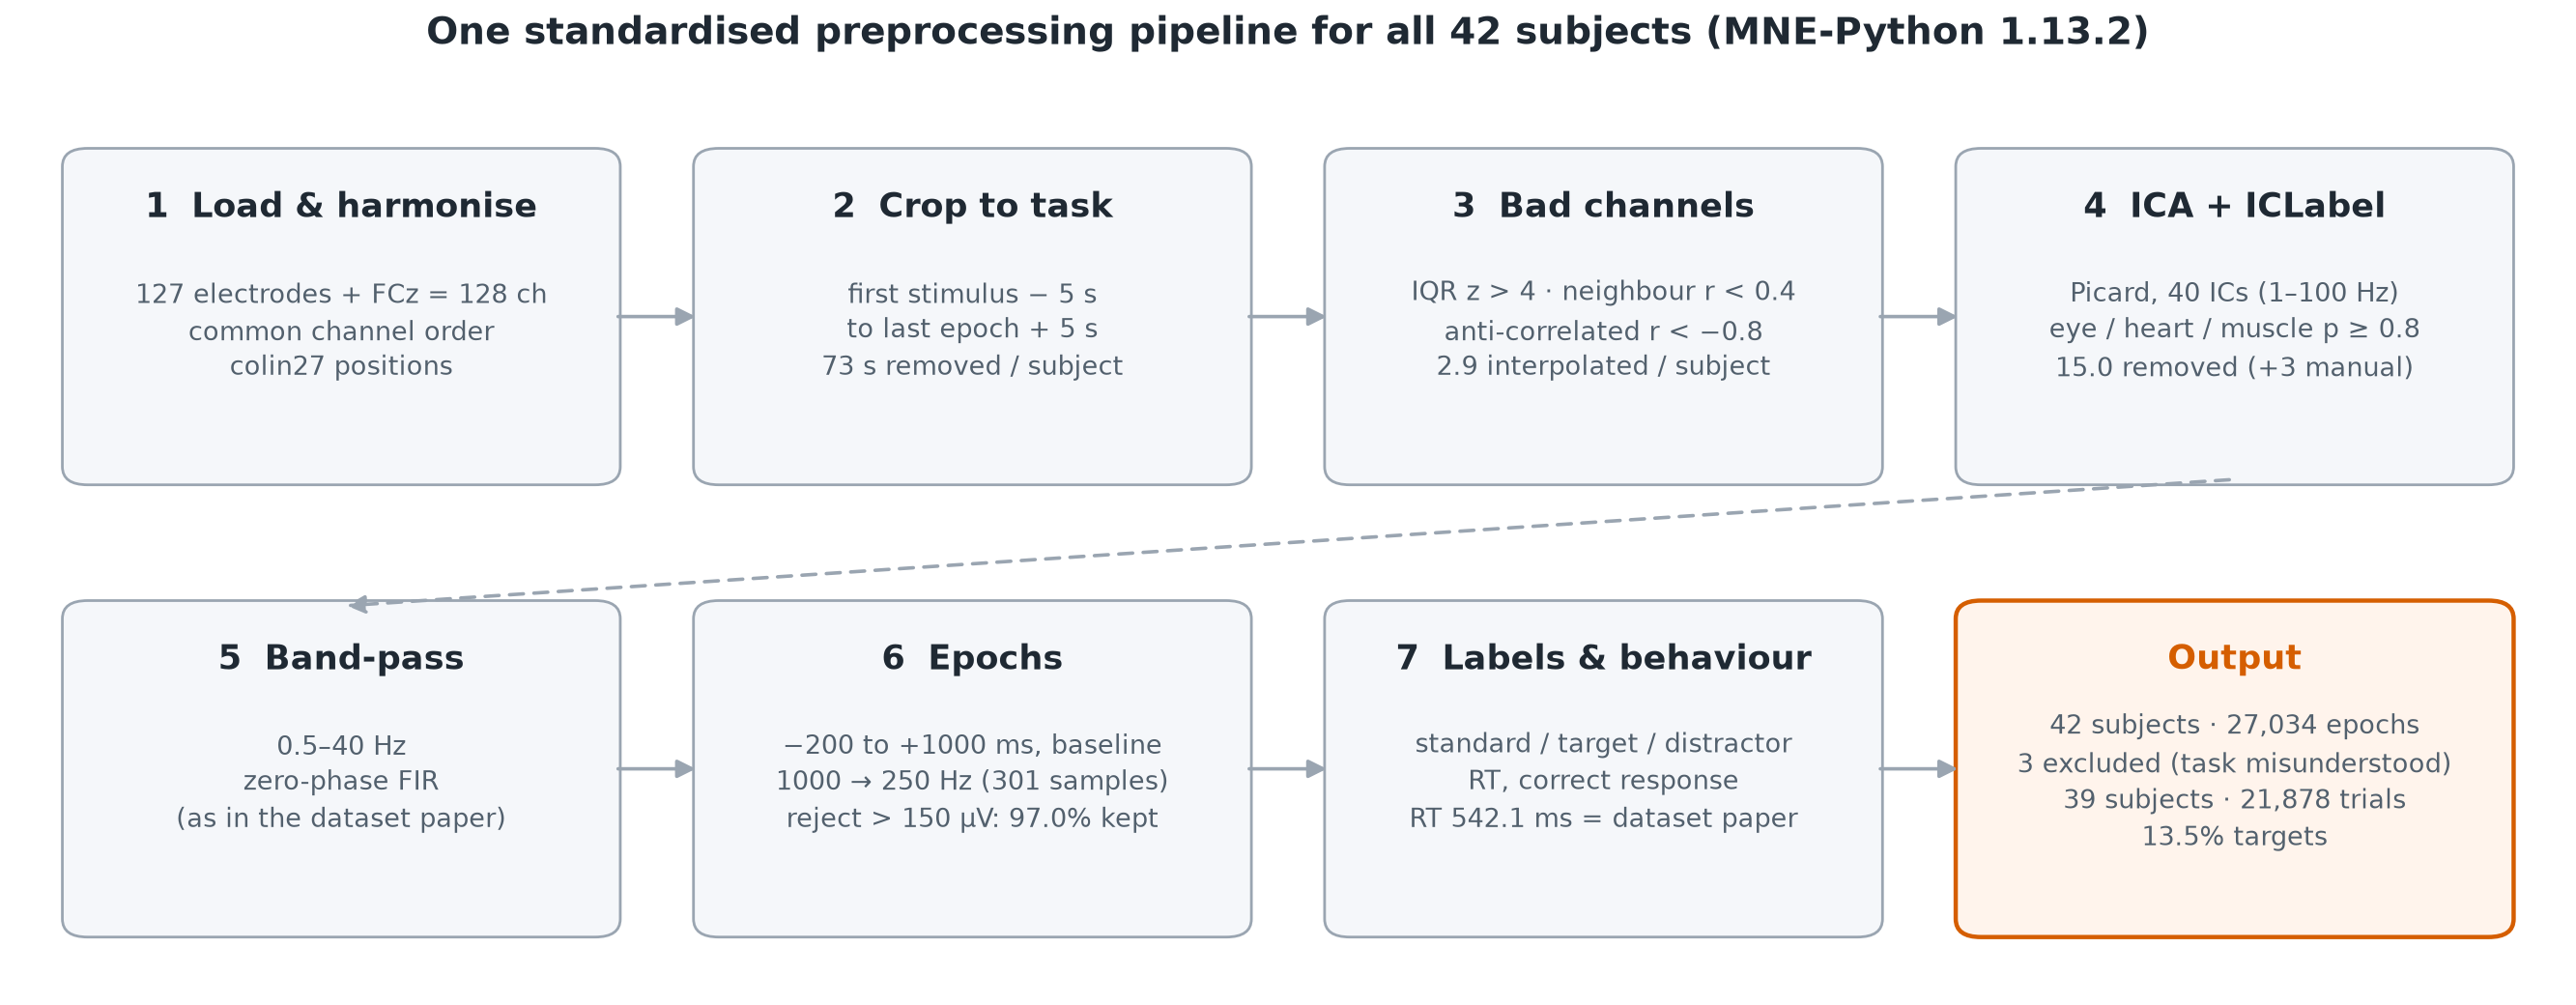
\includegraphics[width=0.92\linewidth,height=28mm,keepaspectratio]{v2_preprocessing_pipeline.png}
  \end{center}
  \vspace{-2mm}
  \begin{columns}[T,onlytextwidth]
    \begin{column}{0.48\textwidth}
      \textbf{Preprocessing steps (in order)}
      \begin{itemize}
        \setlength{\itemsep}{0.6mm}
        \scriptsize
        \item Crop to task, add FCz (128~ch), interpolate bad channels (IQR/corr.), average reference.
        \item Picard ICA (40~ICs) + ICLabel ($p \ge 0.8$, +3 manual blink ICs) for ocular/muscle/cardiac artifacts.
        \item Zero-phase FIR bandpass (0.5--40~Hz) and apply ICA.
        \item Epochs [$-200, +1000$]~ms (250~Hz), baseline [$-200, 0$]~ms, reject $>150\,\mu\text{V}$ ptp.
      \end{itemize}
    \end{column}
    \begin{column}{0.48\textwidth}
      \textbf{Cohort quality control}
      \begin{itemize}
        \setlength{\itemsep}{0.6mm}
        \scriptsize
        \item Artifact rejection retained 27,034/27,865 epochs (97.0\%) across all 42 participants.
        \item Excluded sub-02, sub-14, sub-17 for task misunderstanding (76.5--98.8\% distractor false alarms; mean 91.0\%).
        \item Classification set: 21,878 correct binary trials (39 participants): 18,927 standards, 2,951 targets (13.49\%).
      \end{itemize}
    \end{column}
  \end{columns}
  \vspace{1.2mm}
  \source{Figure 1: Preprocessing pipeline applied identically to all 42 BrainVision recordings}
\end{frame}

% ==============================================================================
% SLIDE 6: SPATIOTEMPORAL DYNAMICS & TOPOMAPS
% ==============================================================================
\begin{frame}{Group scalp topography and individual variability}
  \framesubtitle{128-channel mean potentials (300--500~ms) and cross-subject P300 timing}
  \begin{center}
    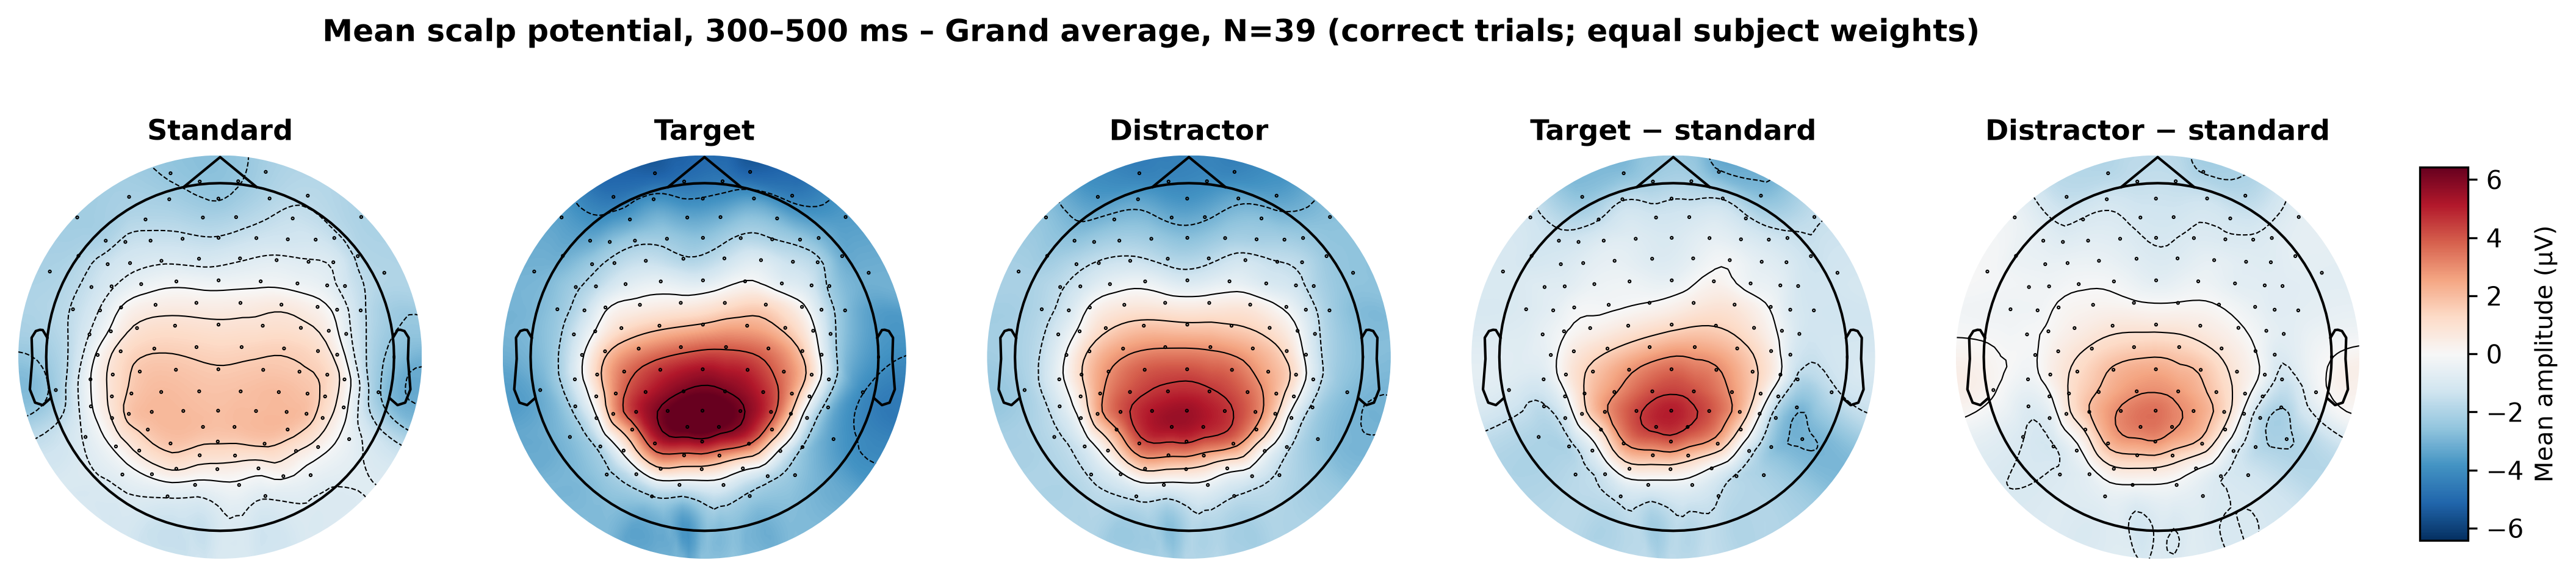
\includegraphics[width=0.95\linewidth,height=32mm,keepaspectratio]{grand_average_p300_summary_topomap.png}
  \end{center}
  \vspace{-1.5mm}
  \begin{columns}[T,onlytextwidth]
    \begin{column}{0.48\textwidth}
      \textbf{Topographic findings (300--500~ms)}
      \begin{itemize}
        \setlength{\itemsep}{0.6mm}
        \scriptsize
        \item Target $-$ standard exhibits a focal parietal maximum around Pz and CPz.
        \item Distractor $-$ standard is also predominantly parietal, with a modest relative frontal shift vs.\ targets (26/39).
        \item Consistent with easy discrimination (5.6\% target misses, 0.27\% standard false alarms).
      \end{itemize}
    \end{column}
    \begin{column}{0.48\textwidth}
      \textbf{Operational P300 checks ($N=39$)}
      \begin{itemize}
        \setlength{\itemsep}{0.6mm}
        \scriptsize
        \item Target $Pz > Fz$: 39/39; oddball contrast $\ge 1.5\,\mu\text{V}$: 37/39.
        \item Independent 200--800~ms peak search: 22/39 peak within 300--500~ms; 17/39 peak later (508--748~ms).
        \item Widening acceptance to 300--600~ms raises core pass rate to 32/39 (motivating 300--600~ms P3 features).
      \end{itemize}
    \end{column}
  \end{columns}
  \vspace{1.2mm}
  \source{Figure 3: Grand average scalp potentials and difference maps in 300--500~ms (checks from Table 4)}
\end{frame}

% ==============================================================================
% SLIDE 7: MACHINE LEARNING BASELINE
% ==============================================================================
\renewcommand{\sectionindex}{04}
\begin{frame}{Conventional machine learning baseline with 402 features}
  \framesubtitle{Extensive feature engineering based on Laton et al. 2014 and time-frequency descriptors}
  \begin{columns}[c,onlytextwidth]
    \begin{column}{0.42\textwidth}
      \textbf{402 features across 12 channels}
      \begin{itemize}
        \setlength{\itemsep}{0.9mm}
        \scriptsize
        \item 120 window amplitude means and SDs (5 latency windows).
        \item 36 P300 peak amp., latency, and area (300--600 ms) + 18 N1/P2/N2 peaks (Fz/Cz/Pz) + 12 peak-to-peak (200--700 ms).
        \item 48 db4 wavelet summaries (300--600 ms): energies (0--8, 8--16, 16--31 Hz) and delta--theta mean.
        \item 36 Hjorth parameters (activity, mobility, complexity).
        \item 132 Welch spectral features: abs./rel. powers (delta--beta), band ratios, and spectral entropy.
      \end{itemize}
      \vspace{1.2mm}
      \textbf{Validation scheme}
      \begin{itemize}
        \setlength{\itemsep}{0.9mm}
        \scriptsize
        \item 5-fold participant-wise GroupKFold.
        \item Inside-fold StandardScaler (for LDA, LR, SVM).
      \end{itemize}
    \end{column}
    \begin{column}{0.56\textwidth}
      \begin{center}
        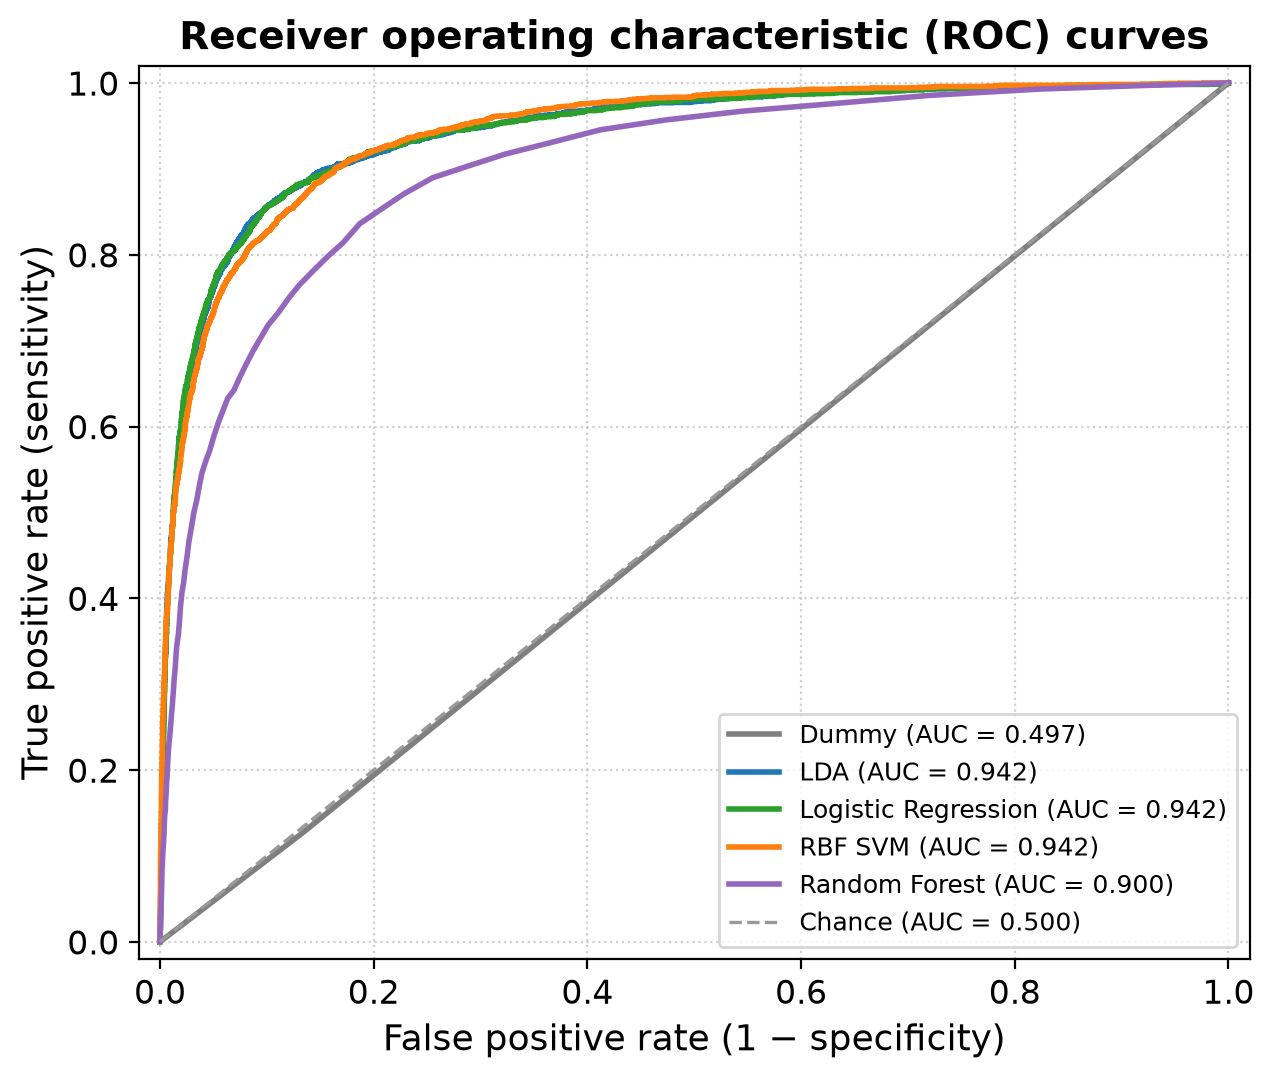
\includegraphics[width=0.98\linewidth,height=52mm,keepaspectratio]{baseline_roc_curves.png}
      \end{center}
      \source{Figure 5: Pooled out-of-fold ROC curves for conventional baseline classifiers}
    \end{column}
  \end{columns}
\end{frame}

% ==============================================================================
% SLIDE 8: EEGNET ARCHITECTURE
% ==============================================================================
\begin{frame}{Compact deep learning architecture: EEGNet-8,2}
  \framesubtitle{End-to-end spatiotemporal convolutional representation on preprocessed 128-channel epochs}
  \begin{columns}[c,onlytextwidth]
    \begin{column}{0.42\textwidth}
      \textbf{EEGNet-8,2 specification}
      \begin{itemize}
        \setlength{\itemsep}{1.3mm}
        \scriptsize
        \item Input: preprocessed 128-channel $\times$ 301-sample epoch at 250 Hz (before feature engineering).
        \item Temporal convolution: 8 filters of kernel length 125 (500 ms).
        \item Depthwise spatial convolution: 16 spatial filters (multiplier $D=2$) across 128 channels.
        \item Separable convolution: depthwise ($1\times16$) and pointwise ($1\times1$) to 16 maps.
        \item Regularization: max-norm constraints (1.0 spatial, 0.25 dense) and dropout ($p=0.5$).
        \item Compact 3,930 trainable parameters; Adam ($\text{lr}=10^{-3}$), class-weighted cross-entropy, patience 15.
      \end{itemize}
    \end{column}
    \begin{column}{0.56\textwidth}
      \begin{center}
        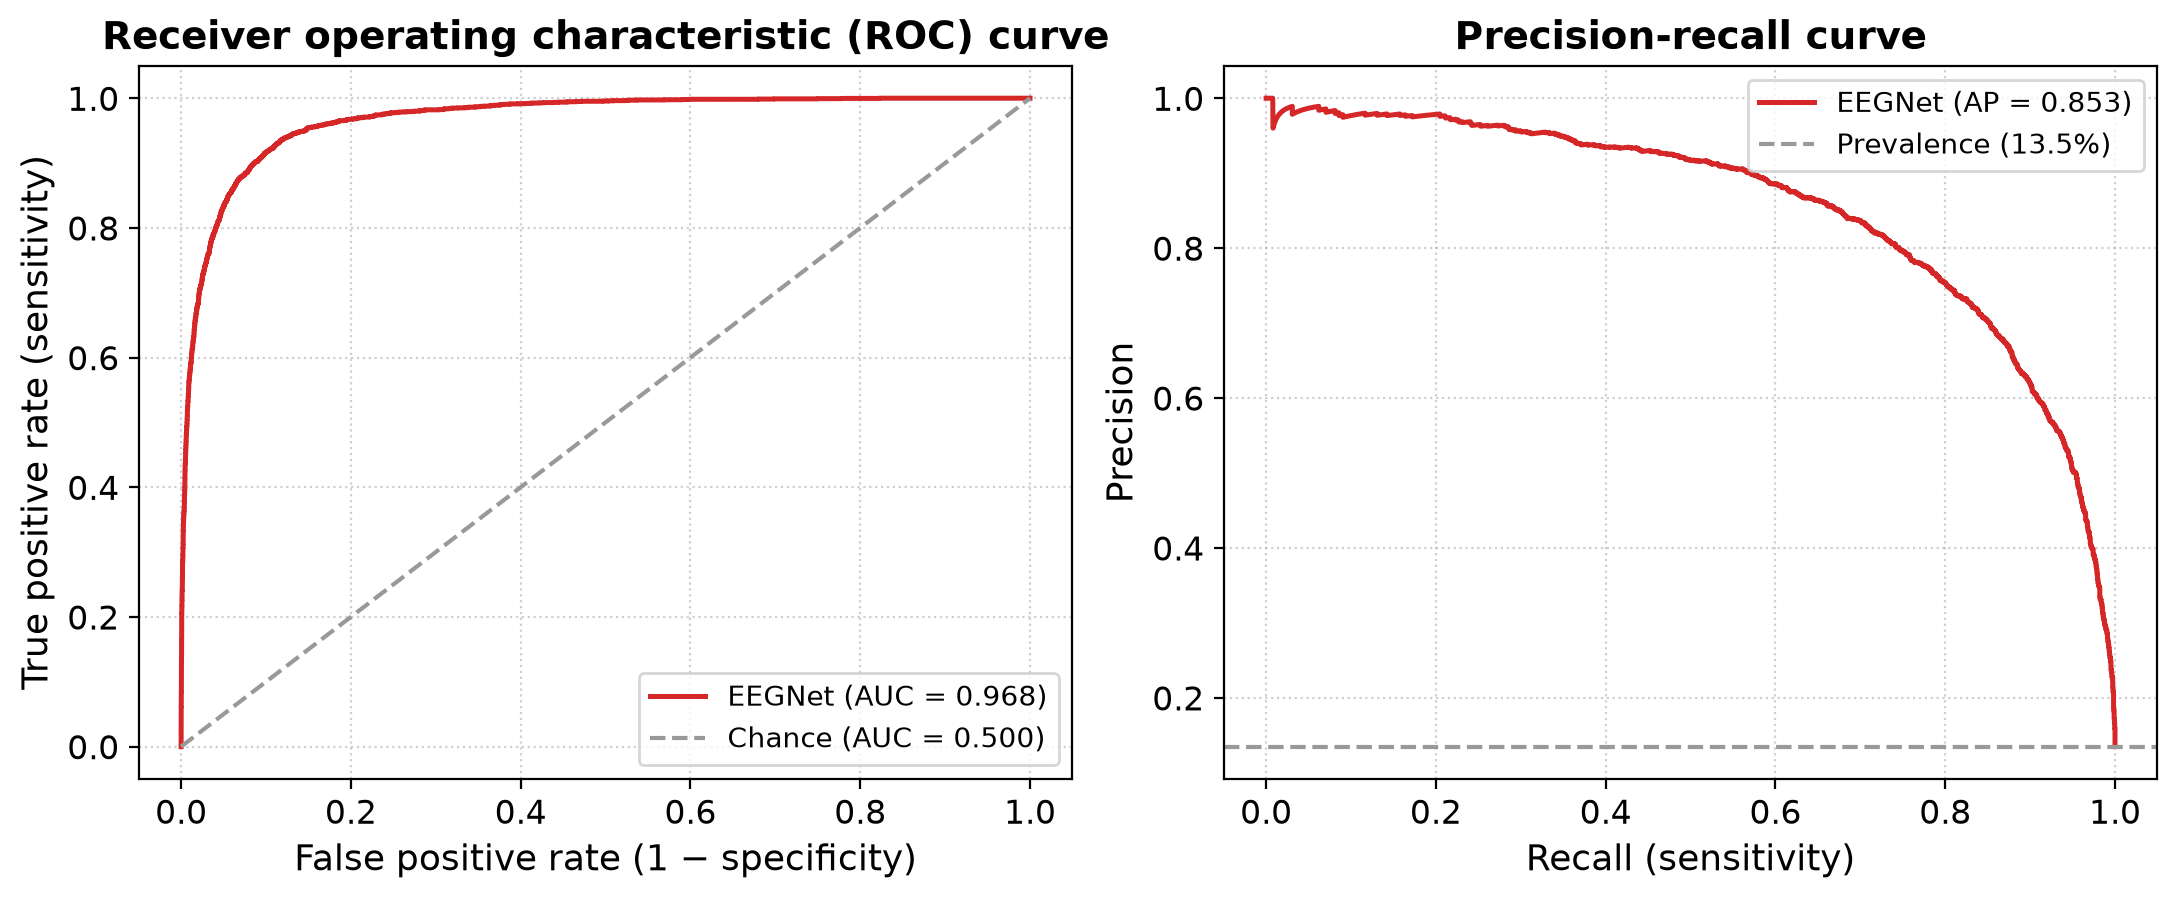
\includegraphics[width=0.98\linewidth,height=52mm,keepaspectratio]{eegnet_roc_pr_real.png}
      \end{center}
      \source{Figure 6: EEGNet pooled out-of-fold ROC and precision-recall curves}
    \end{column}
  \end{columns}
\end{frame}

% ==============================================================================
% SLIDE 9: RESEARCH QUESTION 1 (DIRECT ANSWER)
% ==============================================================================
\begin{frame}{Research question 1: best single-trial classification}
  \framesubtitle{Benchmark comparison across five outer test folds on 21,878 single trials}
  \begin{center}
    \renewcommand{\arraystretch}{1.25}
    \scriptsize
    \begin{tabular}{lcccc}
      \toprule
      Model & Balanced accuracy & ROC-AUC & Average precision & Macro-F1 \\
      \midrule
      Dummy classifier & $0.497 \pm 0.005$ & $0.497 \pm 0.005$ & $0.134 \pm 0.004$ & $0.497 \pm 0.005$ \\
      Random forest & $0.638 \pm 0.041$ & $0.907 \pm 0.025$ & $0.652 \pm 0.046$ & $0.678 \pm 0.053$ \\
      RBF SVM & $0.799 \pm 0.056$ & $0.946 \pm 0.016$ & $0.791 \pm 0.045$ & $0.824 \pm 0.043$ \\
      Shrinkage-LDA & $0.815 \pm 0.060$ & $0.947 \pm 0.022$ & $0.791 \pm 0.075$ & $0.835 \pm 0.045$ \\
      Logistic regression & $0.875 \pm 0.037$ & $0.946 \pm 0.021$ & $0.791 \pm 0.073$ & $0.817 \pm 0.029$ \\
      \midrule
      EEGNet-8,2 & $\mathbf{0.903 \pm 0.021}$ & $\mathbf{0.970 \pm 0.013}$ & $\mathbf{0.865 \pm 0.045}$ & $\mathbf{0.852 \pm 0.030}$ \\
      \bottomrule
    \end{tabular}
  \end{center}
  \vspace{1.5mm}
  \textbf{Direct answer to research question 1}
  \begin{itemize}
    \setlength{\itemsep}{1.5mm}
    \scriptsize
    \item Best overall single-trial model is \textbf{EEGNet-8,2}, reaching ROC-AUC $0.970 \pm 0.013$, average precision $0.865 \pm 0.045$, and balanced accuracy $0.903 \pm 0.021$.
    \item Best linear conventional model is \textbf{shrinkage-LDA} in ROC-AUC ($0.947 \pm 0.022$) and \textbf{logistic regression} in balanced accuracy ($0.875 \pm 0.037$).
    \item At threshold 0.5 under 13.5\% target prevalence, empirical priors and calibration lower sensitivity for LDA (65.9\%), RBF SVM (62.5\%), and Random Forest (28.9\%, specificity 98.8\%); threshold-free ROC-AUC and AP are therefore the fairest ranking comparisons.
  \end{itemize}
  \source{Table 6: Five-fold participant-wise cross-validation results across 39 participants}
\end{frame}

% ==============================================================================
% SLIDE 10: RESEARCH QUESTION 2 (DIRECT ANSWER & CHANNEL CONTROL)
% ==============================================================================
\begin{frame}{Research question 2: deep learning versus machine learning}
  \framesubtitle{Deep learning improves classification, but gain is modest due to P300 linearity}
  \begin{columns}[c,onlytextwidth]
    \begin{column}{0.48\textwidth}
      \begin{center}
        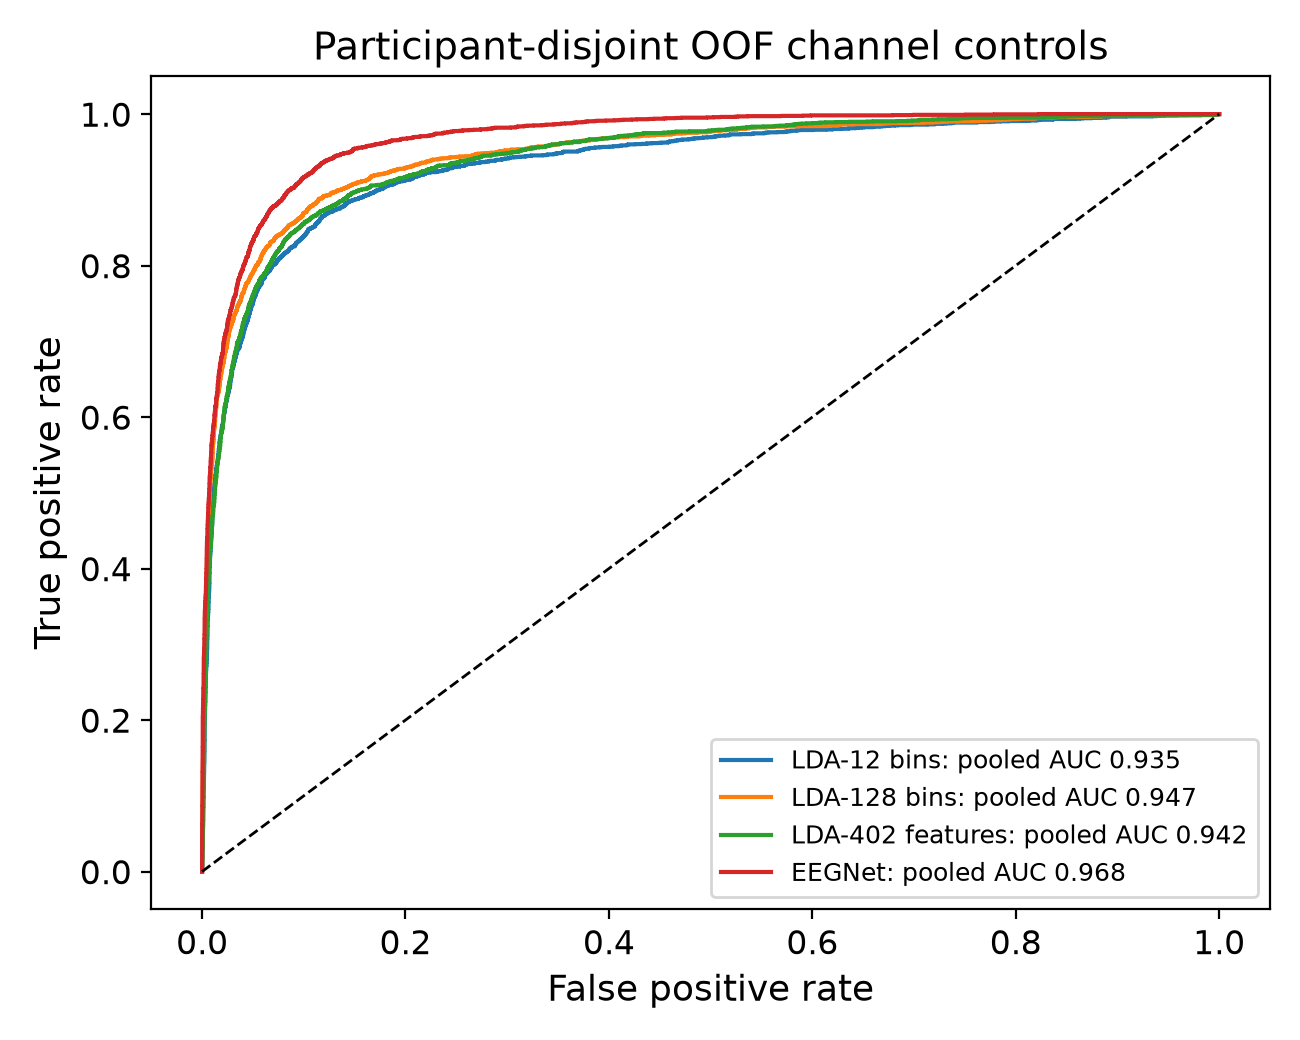
\includegraphics[width=0.98\linewidth,height=50mm,keepaspectratio]{lda_channel_controls_roc.png}
      \end{center}
      \source{Figure 7: Channel-matched LDA controls vs. EEGNet ROC curves}
    \end{column}
    \begin{column}{0.50\textwidth}
      \textbf{Channel-matched evaluation (100 ms bins)}
      \begin{center}
        \renewcommand{\arraystretch}{1.15}
        \scriptsize
        \begin{tabular}{lccc}
          \toprule
          Model and input & Bal. acc. & ROC-AUC & AP \\
          \midrule
          LDA 12 ch (144 feat.) & 0.804 & 0.937 & 0.774 \\
          LDA 128 ch (1,536 feat.) & 0.830 & 0.949 & 0.821 \\
          EEGNet 128 channels & \textbf{0.903} & \textbf{0.970} & \textbf{0.865} \\
          \bottomrule
        \end{tabular}
      \end{center}
      \vspace{1mm}
      \textbf{Direct answer to research question 2}
      \begin{itemize}
        \setlength{\itemsep}{1.1mm}
        \scriptsize
        \item \textbf{Yes, for the tested pipelines}: EEGNet outperforms 402-feature LDA by $+0.023$ ROC-AUC (exploratory Wilcoxon $p = 5.0 \times 10^{-10}$, 35/39 subjects) and $+0.074$ AP.
        \item \textbf{Electrode count alone does not explain gain}: 128-channel LDA reaches 0.949 ($+0.012$ over 12-ch), leaving a $+0.021$ AUC ($+0.043$ AP) margin for EEGNet.
        \item \textbf{Why gain is modest}: P300 behaves as a low-dimensional, largely linear spatio-temporal pattern; shrinkage LDA already captures most separable information, while EEGNet refines spatial--temporal filtering (Blankertz et al., 2011; Lotte et al., 2018).
      \end{itemize}
    \end{column}
  \end{columns}
\end{frame}

% ==============================================================================
% SLIDE 11: DISTRACTOR CONTROL (NO-BUTTON EXPERIMENT)
% ==============================================================================
\begin{frame}{No-button distractor control}
  \framesubtitle{Testing whether EEGNet can decode rare stimuli without a motor-response contrast}
  \begin{columns}[c,onlytextwidth]
    \begin{column}{0.54\textwidth}
      \begin{center}
        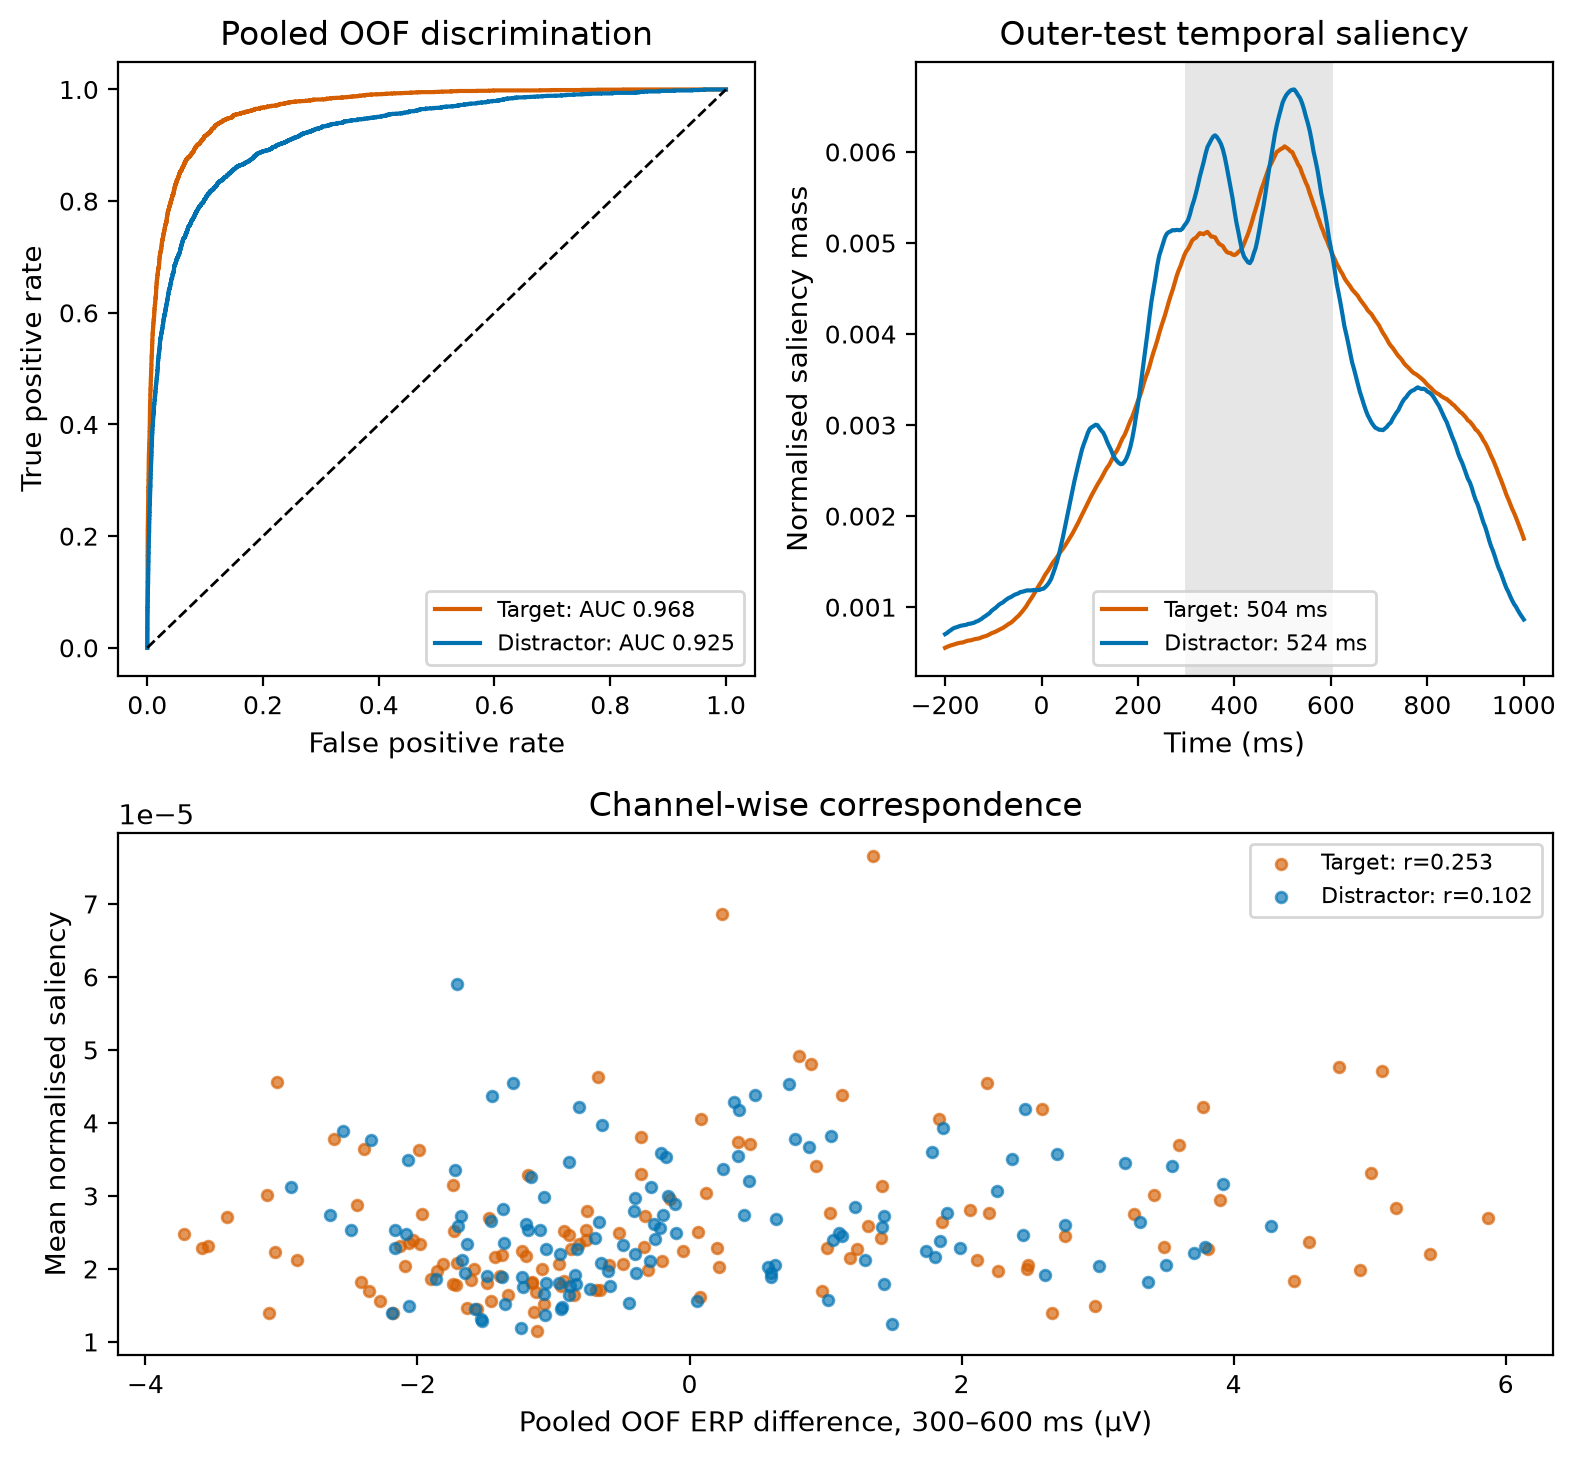
\includegraphics[width=0.98\linewidth,height=50mm,keepaspectratio]{eegnet_controls_oof.png}
      \end{center}
      \source{Figure 8: Out-of-fold ROC, temporal saliency, and channel-wise correspondence for both tasks}
    \end{column}
    \begin{column}{0.44\textwidth}
      \textbf{Distractor versus standard control}
      \begin{itemize}
        \setlength{\itemsep}{1.4mm}
        \scriptsize
        \item Target trials require a button press, introducing potential motor-related cues.
        \item Five matched EEGNet models were trained on correct distractor vs.\ standard trials (21,748 trials; identical outer test folds).
        \item Neither class involves a button response (verified from metadata).
      \end{itemize}
      \vspace{1.2mm}
      \textbf{Control results and scope}
      \begin{itemize}
        \setlength{\itemsep}{1.3mm}
        \scriptsize
        \item ROC-AUC: \mbox{\textbf{0.926 $\pm$ 0.015}}; Bal.\ acc.: \mbox{\textbf{0.855 $\pm$ 0.020}}; AP: \mbox{\textbf{0.745 $\pm$ 0.048}}.
        \item Shows EEGNet can discriminate rare stimuli without a button-press contrast.
        \item \textbf{Scope caveat}: does not quantify target motor share --- stimulus identity, task relevance, and ERP shape also differ.
      \end{itemize}
    \end{column}
  \end{columns}
\end{frame}

% ==============================================================================
% SLIDE 12: RESEARCH QUESTION 3 (SALIENCY & INTERPRETABILITY)
% ==============================================================================
\begin{frame}{Research question 3: outer-test gradient saliency}
  \framesubtitle{Partial physiological correspondence alongside sensorimotor, anterior, and visual sensitivity}
  \begin{columns}[c,onlytextwidth]
    \begin{column}{0.52\textwidth}
      \begin{center}
        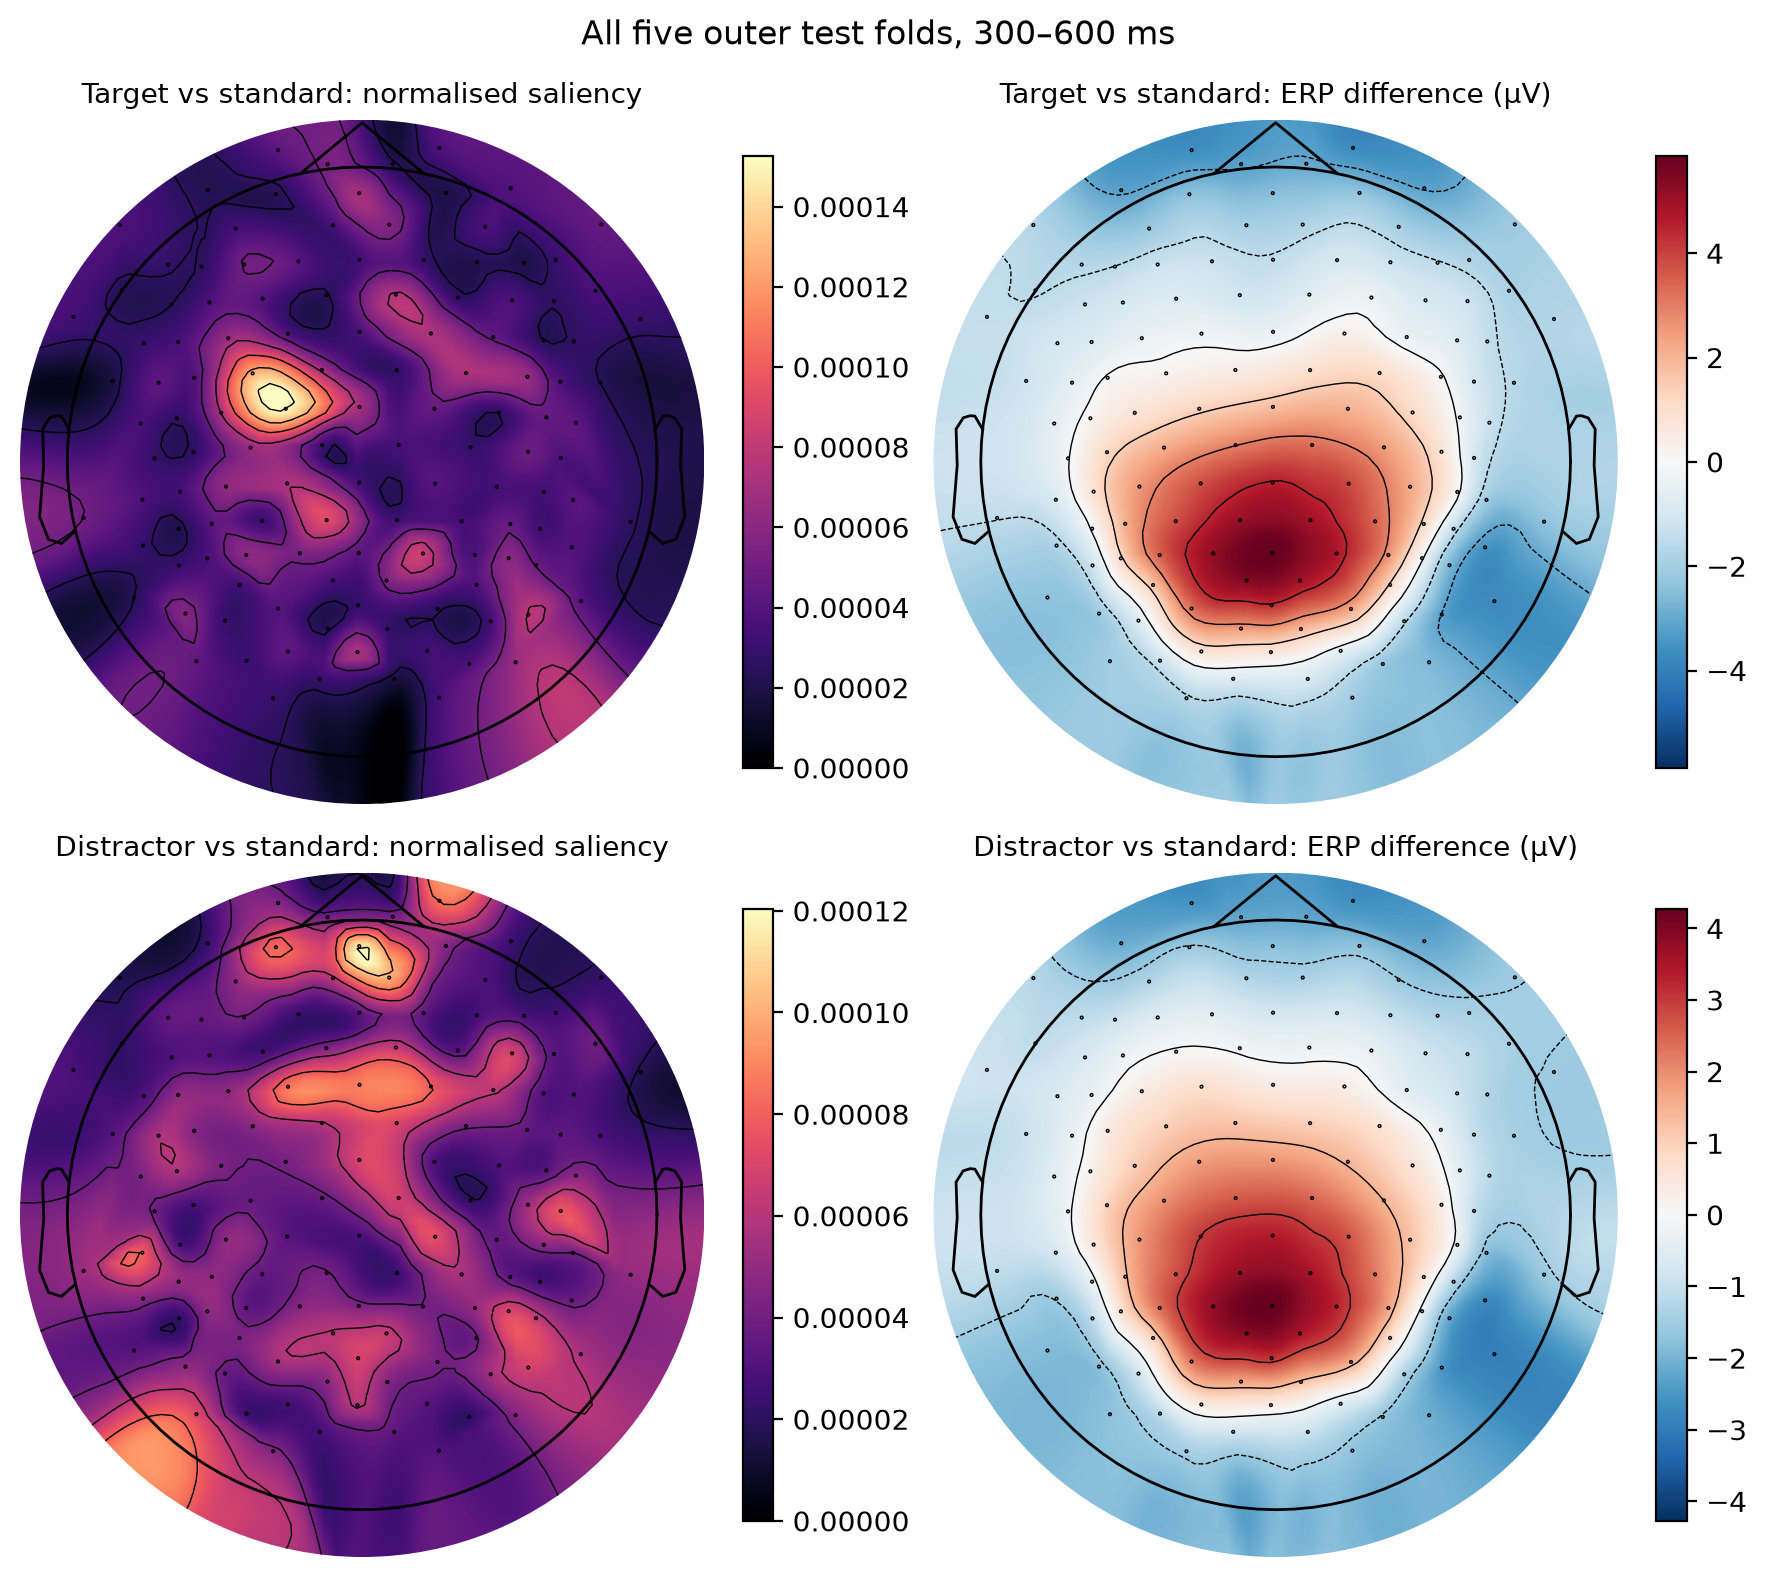
\includegraphics[width=0.98\linewidth,height=50mm,keepaspectratio]{eegnet_controls_topomaps.png}
      \end{center}
      \source{Figure 9: Saliency topomaps (300--600~ms) and ERP voltage differences for both tasks}
    \end{column}
    \begin{column}{0.46\textwidth}
      \textbf{Direct answer to research question 3}
      \begin{itemize}
        \setlength{\itemsep}{1.1mm}
        \scriptsize
        \item \textbf{Partly interpretable}: computed strictly on positive outer-test trials (all 5 folds, L1-normalised before pooling).
        \item \textbf{Target temporal alignment}: peak at 504~ms (near 542.1~ms mean RT), 40.7\% mass in 300--600~ms (1.61$\times$ uniform).
        \item \textbf{Partial spatial match}: $r = 0.253$ full-epoch ($0.203$ in 300--600~ms; fold range 0.057--0.289); Pz ranks 43/128; top sites are left-central (C1, FCC3h, C3) + Oz, P2.
        \item \textbf{Distractor shift}: peak 524~ms (43.9\%); left-central cluster vanishes ($r = 0.102$, Pz rank 56/128), shifting to anterior sites (AFz, AFF2h, FC1, AF3 --- possible residual ocular signal) and Oz ($\sim$100~ms visual peak).
        \item \textbf{Caution}: input gradients measure local predictive sensitivity, not neural sources (Haufe et al., 2014).
      \end{itemize}
    \end{column}
  \end{columns}
\end{frame}

% ==============================================================================
% SLIDE 13: SUMMARY TABLE OF THE 3 RESEARCH QUESTIONS
% ==============================================================================
\renewcommand{\sectionindex}{05}
\begin{frame}{Summary of answers to the three research questions}
  \framesubtitle{Evidence-based synthesis aligned with the final report}
  \begin{center}
    \renewcommand{\arraystretch}{1.3}
    \scriptsize
    \begin{tabularx}{\linewidth}{l>{\raggedright\arraybackslash}X>{\raggedright\arraybackslash}p{46mm}}
      \toprule
      Question & Core quantitative evidence & Neuroscientific and ML rationale \\
      \midrule
      \textbf{RQ1: Best single-trial result} &
      EEGNet achieves ROC-AUC $0.970 \pm 0.013$, average precision $0.865 \pm 0.045$, and balanced accuracy $0.903 \pm 0.021$. Best linear baselines: shrinkage-LDA (AUC 0.947) and LR (Bal.\ acc.\ 0.875). &
      End-to-end spatiotemporal filters learn directly from preprocessed 128-ch epochs without fixed latency-window loss. \\
      \midrule
      \textbf{RQ2: Is deep learning better?} &
      \textbf{Yes, for tested pipelines}: $+0.023$ ROC-AUC over 402-feature LDA (exploratory $p = 5.0 \times 10^{-10}$; 35/39 higher) and $+0.021$ over 128-ch LDA ($+0.043$ AP). &
      P300 behaves as a low-dimensional, largely linear spatio-temporal pattern where shrinkage LDA captures most separable signal; EEGNet refines spatial--temporal filtering. \\
      \midrule
      \textbf{RQ3: Are features explainable?} &
      \textbf{Partly.} Outer-test saliency peaks at 504~ms (40.7\% in 300--600~ms), partial spatial $r = 0.253$ (Pz rank 43/128). No-button distractor reaches 0.926 ROC-AUC ($r = 0.102$). &
      Shows stimulus decoding without a button press, while left-central target sensitivity (C1/C3), distractor anterior/visual cues (AFz/Oz), and Haufe et al.\ (2014) leave exact mechanisms open. \\
      \bottomrule
    \end{tabularx}
  \end{center}
\end{frame}

% ==============================================================================
% SLIDE 14: TEAM CONTRIBUTIONS
% ==============================================================================
\begin{frame}{Team roles and contribution shares}
  \framesubtitle{Strictly compliant with slide 143: individual responsibilities and shares summing to 100\%}
  \begin{center}
    \renewcommand{\arraystretch}{1.2}
    \scriptsize
    \begin{tabularx}{\linewidth}{lXcc}
      \toprule
      Member & Main project responsibilities & Role code & Share \\
      \midrule
      Nguyễn Văn Vũ & Project coordination, dataset management, documentation, final controls and verification & V1 & 17.67\% \\
      Thái Nguyễn Hoàng Bách & Preprocessing pipeline, Picard ICA, ICLabel artifact review, QC summary & V2 & 11.65\% \\
      Trương Huy Hoàng & ERP waveforms, operational verification, group statistics, visualization & V3 & 17.67\% \\
      Nguyễn Công Kiên & Feature engineering (402 features), time-frequency, db4 wavelet, ranking & V4 & 17.67\% \\
      Nguyễn Việt Đức & Conventional ML pipelines (LDA, SVM, RF, LR), GroupKFold, comparisons & V5 & 17.67\% \\
      Đồng Minh Đức & PyTorch EEGNet-8,2, gradient saliency, ML/DL comparison & V6 & 17.67\% \\
      \midrule
      \multicolumn{2}{l}{\textbf{Total contribution across all group members}} & & \textbf{100.00\%} \\
      \bottomrule
    \end{tabularx}
  \end{center}
  \vspace{1.5mm}
  \takeaway{Fully reproducible repository with automated pipelines, 11 unit tests, and fixed random seeds.}
  \source{Table 12: Member contributions documented in report and contributions log}
\end{frame}

% ==============================================================================
% SLIDE 15: CONCLUSION
% ==============================================================================
\begin{frame}
  \centering
  \vspace{12mm}
  {\color{Navy}\bfseries\fontsize{26}{30}\selectfont
  Thank you for your attention!\par}
  \vspace{7mm}
  {\color{TitleNavy}\fontsize{12}{15}\selectfont
  Single-trial P300 classification project - AIT3012 Neuroscience\par}
  \vspace{4mm}
  {\color{Muted}\small
  VNU University of Engineering and Technology\\
  Institute of Artificial Intelligence\par}
\end{frame}

\end{document}
